\documentclass[a4paper,12pt]{article}

% --- Essential Packages ---
\usepackage[utf8]{inputenc}
\usepackage[T1]{fontenc}
\usepackage[english]{babel}
\usepackage{geometry}
\usepackage{graphicx}
\usepackage{hyperref}
\usepackage{listings}
\usepackage{xcolor}
\usepackage{float}
\usepackage{fancyhdr}
\usepackage{titlesec}
\usepackage{enumitem}
\usepackage{booktabs}
\usepackage{parskip}
\usepackage{tikz}
\usepackage{adjustbox}
\usetikzlibrary{shapes.geometric, arrows.meta, positioning, fit, backgrounds, calc}

% --- Page Configuration ---
\geometry{margin=2.5cm, top=3cm, bottom=3cm}

% --- Color Scheme ---
\definecolor{codegray}{gray}{0.95}

% --- Hyperlink Configuration ---
\hypersetup{
    colorlinks=true,
    linkcolor=black,
    urlcolor=black,
    citecolor=black,
    pdftitle={Design Document - Concurrent HTTP Web Server},
    pdfauthor={Martim Gil, Nuno Leite Faria}
}

% --- Code Style ---
\lstset{
    backgroundcolor=\color{codegray},
    basicstyle=\ttfamily\small,
    breaklines=true,
    frame=single,
    framerule=0.5pt,
    rulecolor=\color{black},
    numbers=left,
    numberstyle=\tiny,
    captionpos=b,
    keywordstyle=\bfseries,
    commentstyle=\itshape,
    stringstyle=\ttfamily,
    showstringspaces=false,
    tabsize=4,
    xleftmargin=1em,
    xrightmargin=1em,
    aboveskip=1em,
    belowskip=1em,
    language=C
}

% --- Header and Footer ---
\setlength{\headheight}{14pt}
\pagestyle{fancy}
\fancyhf{}
\fancyhead[L]{\small\textit{Concurrent HTTP Web Server}}
\fancyhead[R]{\small\textit{Design Document}}
\fancyfoot[C]{\thepage}
\renewcommand{\headrulewidth}{0.4pt}
\renewcommand{\footrulewidth}{0pt}

% --- Section Styling ---
\titleformat{\section}{\Large\bfseries}{\thesection}{1em}{}
\titleformat{\subsection}{\large\bfseries}{\thesubsection}{1em}{}
\titleformat{\subsubsection}{\normalsize\bfseries}{\thesubsubsection}{1em}{}

% --- List Styling ---
\setlist[itemize]{noitemsep, topsep=0.5em}
\setlist[enumerate]{noitemsep, topsep=0.5em}

\begin{document}

% =================================================================
% TITLE PAGE
% =================================================================
\begin{titlepage}
    \centering
    
    % --- DETI Logo ---
    \vspace*{2cm}
    \includegraphics[width=0.7\textwidth]{deti.png}
    
    \vspace{3cm}
    
    % --- Document Title ---
    {\Huge\textbf{Design Document}}\\[0.5cm]
    {\LARGE Concurrent HTTP Web Server}
    
    \vspace{1.5cm}
    
    % --- Decorative Line ---
    \rule{0.6\textwidth}{0.5pt}
    
    \vspace{1.5cm}
    
    % --- Course Information ---
    {\Large\textbf{Operating Systems}}\\[0.3cm]
    {\large Academic Year 2024/2025}
    
    \vspace{2cm}
    
    % --- Authors ---
    \begin{tabular}{cc}
        \textbf{Martim Gil} & \textbf{Nuno Leite Faria} \\
        Student ID: 124833 & Student ID: 112994 \\
    \end{tabular}
    
    \vspace{1.5cm}
    
    % --- Supervisor ---
    {\large Supervisor: Prof. Pedro Azevedo Fernandes}
    
    \vfill
    
    % --- Date ---
    {\large \today}
    
\end{titlepage}

% --- Table of Contents ---
\tableofcontents
\newpage
    
    % ----------------------------------------------------------------------
    \section{Architecture Overview}
    % ----------------------------------------------------------------------
    
    The system adopts a multi-process, multi-threaded architecture based on a
    Master–Worker model. This structure enables efficient handling of multiple
    simultaneous client connections while preserving process isolation and
    scalability across CPU cores.
    
    \subsection{Process Model}
    
    The application consists of one \textbf{Master Process} and $N$ \textbf{Worker Processes}.
    Each performs a distinct role in the server’s execution pipeline:
    
    \begin{itemize}
        \item \textbf{Master:} Initializes configuration parameters, binds the listening
              socket, and accepts incoming TCP connections. Each accepted connection
              is first represented as a descriptor stored in a bounded
              shared-memory queue, protected by semaphores. The master then transfers
              the corresponding client file descriptor to the designated worker via
              a UNIX domain socket using \texttt{SCM\_RIGHTS}. This approach
              combines efficient interprocess signaling with safe descriptor passing.
        \item \textbf{Workers:} Spawned by the master at startup, each worker waits for
              connection assignments in the shared queue. Upon notification, it
              receives the actual socket descriptor through the UNIX channel and
              submits it to its local thread pool for processing. Each worker
              maintains its own cache and counters but contributes to global
              statistics through synchronized shared memory updates.
    \end{itemize}
    
\begin{figure}[H]
    \centering
    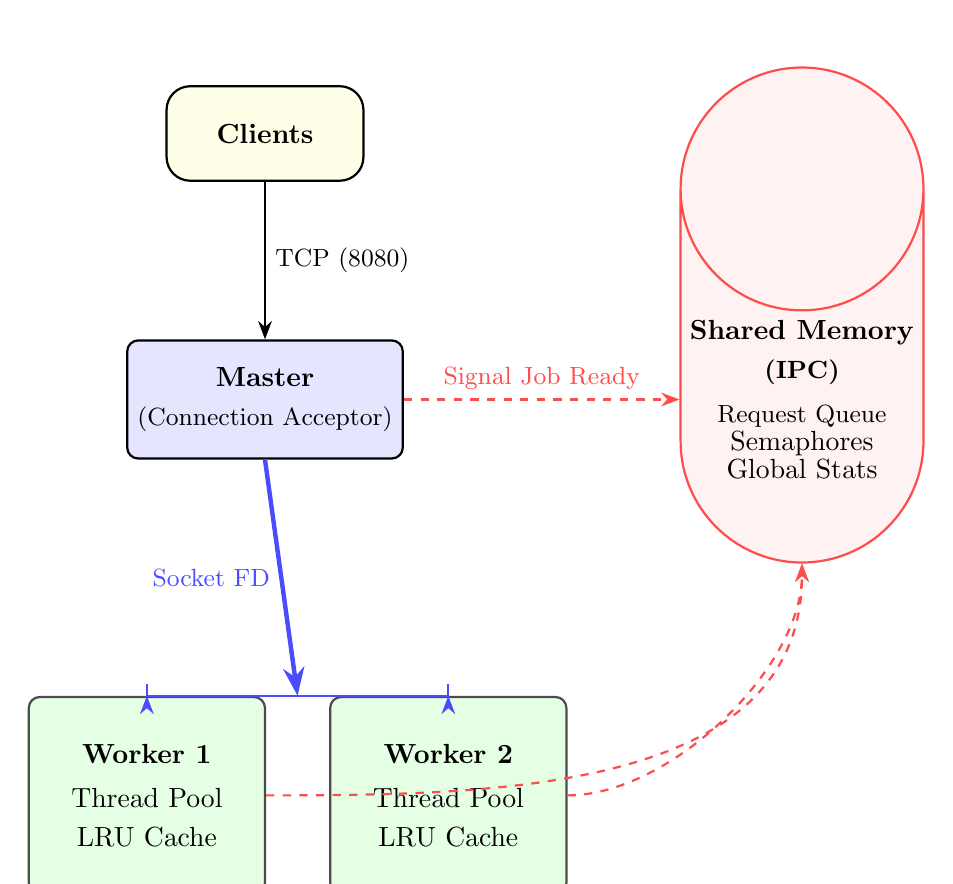
\begin{tikzpicture}[
        process/.style={rectangle, draw=black, thick, fill=blue!10, minimum width=3.5cm, minimum height=1.5cm, align=center, rounded corners, font=\normalsize},
        worker/.style={rectangle, draw=black!70, thick, fill=green!10, minimum width=3cm, minimum height=2.5cm, align=center, rounded corners, font=\normalsize},
        shm/.style={cylinder, shape border rotate=90, draw=red!70, thick, fill=red!5, minimum width=3cm, minimum height=3.5cm, align=center, font=\normalsize},
        comp/.style={rectangle, draw=gray, dashed, fill=white, font=\small, minimum width=2cm, minimum height=0.5cm, align=center},
        cloudnode/.style={rectangle, draw=black, thick, fill=yellow!10, minimum width=2.5cm, minimum height=1.2cm, align=center, rounded corners=0.3cm, font=\normalsize},
        arrow/.style={->, >=Stealth, thick}
    ]

    % Master Process
    \node (master) [process] {\textbf{Master}\\[2pt]\small(Connection Acceptor)};

    % Shared Memory 
    \node (shm) [shm, right=3.5cm of master] {
        \textbf{Shared Memory}\\[2pt]\small\textbf{(IPC)}\\[4pt]
        \small Request Queue\\[-2pt]
        Semaphores\\[-2pt]
        Global Stats
    };
    
    % Workers
    \node (worker1) [worker, below=3cm of master, xshift=-1.5cm] {
        \textbf{Worker 1}\\[4pt]
        Thread Pool\\[2pt]
        LRU Cache
    };

    \node (worker2) [worker, right=0.8cm of worker1] {
        \textbf{Worker 2}\\[4pt]
        Thread Pool\\[2pt]
        LRU Cache
    };

    % Clients
    \node (client) [cloudnode, above=2cm of master] {\textbf{Clients}};

    % Edges
    \draw[arrow] (client) -- node[right, font=\small] {TCP (8080)} (master);

    \draw[arrow, dashed, color=red!70] (master.east) -- (shm.west)
        node[above, midway, font=\small, color=red!70] {Signal Job Ready};

    \draw[arrow, ultra thick, color=blue!70] (master.south) -- 
        node[left, font=\small, color=blue!70] {Socket FD} 
        ($(worker1.north)!0.5!(worker2.north)$);
    
    \draw[arrow, color=blue!70] ($(worker1.north)!0.5!(worker2.north)$) -| (worker1.north);
    \draw[arrow, color=blue!70] ($(worker1.north)!0.5!(worker2.north)$) -| (worker2.north);

    \draw[arrow, dashed, color=red!70] (worker1.east) to[out=0, in=270, looseness=1] (shm.south);
    \draw[arrow, dashed, color=red!70] (worker2.east) to[out=0, in=270, looseness=0.8] (shm.south);

    \end{tikzpicture}
    \caption{System Architecture: Process Model and IPC Coordination}
    \label{fig:arch}
\end{figure}
    
    \subsection{Thread Model}
    
    Within each worker process, a fixed sized pool of threads is created during
    initialization. The pool is managed through a bounded queue protected by a
    \texttt{pthread\_mutex\_t} and a pair of condition variables for signaling.
    Threads block when the queue is empty and wake upon task submission.  
    Each thread handles one complete HTTP request–response cycle before returning
    to the idle state. This design eliminates the overhead of thread creation at
    runtime and maintains steady throughput under heavy load.
    
    \subsection{Coordination and Synchronization}
    
    Interprocess coordination relies on POSIX shared memory and named semaphores.
    Shared memory stores both the connection queue and aggregated statistics,
    while semaphores enforce mutual exclusion and synchronize access between the
    master and workers.  
    Within workers, thread-level synchronization is handled by mutexes and
    condition variables, ensuring safe access to shared structures such as the
    cache and log system. This combination of IPC primitives and in-process
    synchronization guarantees correctness even under high concurrency.
    
    \subsection{Design Rationale}
    
    The architecture separates responsibilities cleanly: the master focuses on
    connection management and system orchestration, while workers specialize in
    request handling. The use of shared memory for lightweight signaling and
    descriptor passing through UNIX domain sockets minimizes communication
    overhead and preserves process isolation.  
    This design yields a scalable, fault-tolerant server capable of leveraging
    multi-core systems effectively while maintaining predictable and stable
    performance.
    
    
    % ----------------------------------------------------------------------
    % 2. SHARED DATA STRUCTURES
    % ----------------------------------------------------------------------
    \section{Shared Data Structures}
    Inter-Process Communication (IPC) between the master and workers relies on
    POSIX shared memory with named semaphores. The shared region holds a
    bounded queue for connection dispatch and a set of global runtime counters.
    
    \subsection{Memory Layout}
    
    Defined in \texttt{shared\_mem.h}, the \texttt{shared\_data\_t} structure
    is allocated by the master process and mapped by all workers.
    
    \begin{lstlisting}[language=C]
    typedef struct {
        request_queue_t queue;   // Connection queue
        server_stats_t  stats;   // Global statistics
    } shared_data_t;
    \end{lstlisting}
    
    Creation uses \texttt{shm\_open()}, \texttt{ftruncate()}, and
    \texttt{mmap()}, with cleanup performed by the master on shutdown
    via \texttt{shm\_unlink()}.
    
    \subsection{Circular Buffer}
    
    The interprocess queue is implemented as a bounded FIFO in shared memory:
    
    \begin{lstlisting}[language=C]
    typedef struct {
        int worker_id;       // Target worker
        int placeholder_fd;  // Marker only (real FD passed via SCM_RIGHTS)
    } connection_item_t;
    
    typedef struct {
        connection_item_t items[MAX_QUEUE_SIZE];
        int front;          // Dequeue index
        int rear;           // Enqueue index
        int count;          // Current occupancy
    } connection_queue_t;
    \end{lstlisting}
    
    \paragraph{Semantics.}\mbox{}\\[-0.2\baselineskip]
    The Master (producer) enqueues a \texttt{connection\_item\_t} selecting the
    \texttt{worker\_id}; the \texttt{placeholder\_fd} is not a transferable descriptor.
    The actual client socket is sent to the chosen Worker over a UNIX domain socket
    using \texttt{SCM\string_RIGHTS}.
    
    \paragraph{Synchronization.}\mbox{}\\[-0.2\baselineskip]
    Enqueue/dequeue follow classical producer--consumer control with named semaphores:
    \texttt{empty\_slots} (free capacity), \texttt{filled\_slots} (pending items),
    and \texttt{queue\_mutex} (exclusive updates of \texttt{front}/\texttt{rear}/\texttt{count}).
    On enqueue: wait \texttt{empty\_slots} $\rightarrow$ lock \texttt{queue\_mutex}
    $\rightarrow$ write \texttt{items[rear]} and advance \texttt{rear} (mod
    \texttt{MAX\_QUEUE\_SIZE}); increment \texttt{count} $\rightarrow$ unlock
    $\rightarrow$ post \texttt{filled\_slots}.  
    On dequeue: wait \texttt{filled\_slots} $\rightarrow$ lock \texttt{queue\_mutex}
    $\rightarrow$ read \texttt{items[front]} and advance \texttt{front}; decrement
    \texttt{count} $\rightarrow$ unlock $\rightarrow$ post \texttt{empty\_slots}.
    This guarantees correctness under concurrent producers/consumers and prevents
    overrun/underrun of the circular buffer.
    
    
    \subsection{Global Statistics}
    
    The \texttt{server\_stats\_t} structure, located in the same region,
    records cumulative server activity.
    
    \begin{lstlisting}[language=C]
    typedef struct {
        long total_requests;          
        long bytes_transferred;        
        long status_200;              
        long status_404;               
        long status_500;            
        int  active_connections;       
        long total_response_time_ms;  
    } server_stats_t;
    \end{lstlisting}
    
    Workers increment these counters under a dedicated semaphore
    (\texttt{stats\_mutex}) to guarantee atomic access.  
    Values are read periodically by monitoring components such as the web
    dashboard and log system.
    
    \subsection{Synchronization Lifecycle}
    
    The master initializes shared memory and all semaphores during startup,
    while workers connect to existing objects.  
    At termination, the master releases all IPC resources, preventing
    persistent semaphores or memory segments.
    
    This design achieves reliable communication and coordinated state
    management with minimal interprocess overhead.
    
    % ----------------------------------------------------------------------
    % 3. SYNCHRONIZATION MECHANISMS
    % ----------------------------------------------------------------------
    \section{Synchronization Mechanisms}
    
    \subsection{Process Synchronization (Named Semaphores)}
    Master and Workers coordinate over a bounded circular queue in shared memory using
    named POSIX semaphores (see \texttt{semaphores.h/.c}, \texttt{shared\_mem.h/.c}):
    
    \begin{itemize}
      \item \textbf{\texttt{empty\_slots}} (\texttt{/ws\_empty}) --- counts free positions in the interprocess queue; the Master (producer) waits when the queue is full.
      \item \textbf{\texttt{filled\_slots}} (\texttt{/ws\_filled}) --- counts pending items. Workers (consumers) wait when the queue is empty.
      \item \textbf{\texttt{queue\_mutex}} (\texttt{/ws\_queue\_mutex}) --- mutual exclusion for updating queue indices (\texttt{front/rear/count}).
      \item \textbf{\texttt{stats\_mutex}} (\texttt{/ws\_stats\_mutex}) --- serializes updates to \texttt{server\_stats\_t} (see \texttt{stats.c}).
      \item \textbf{\texttt{log\_mutex}} (\texttt{/ws\_log\_mutex}) --- serializes log writes across processes.
    \end{itemize}
    
    Producer path (in \texttt{master.c}): wait \texttt{empty\_slots} $\rightarrow$ lock \texttt{queue\_mutex} $\rightarrow$ enqueue $\rightarrow$ unlock $\rightarrow$ post \texttt{filled\_slots}.  
    Consumer path (in \texttt{worker.c}): wait \texttt{filled\_slots} $\rightarrow$ lock \texttt{queue\_mutex} $\rightarrow$ dequeue $\rightarrow$ unlock $\rightarrow$ post \texttt{empty\_slots}.
    
\begin{figure}[H]
\centering
\resizebox{\textwidth}{!}{%
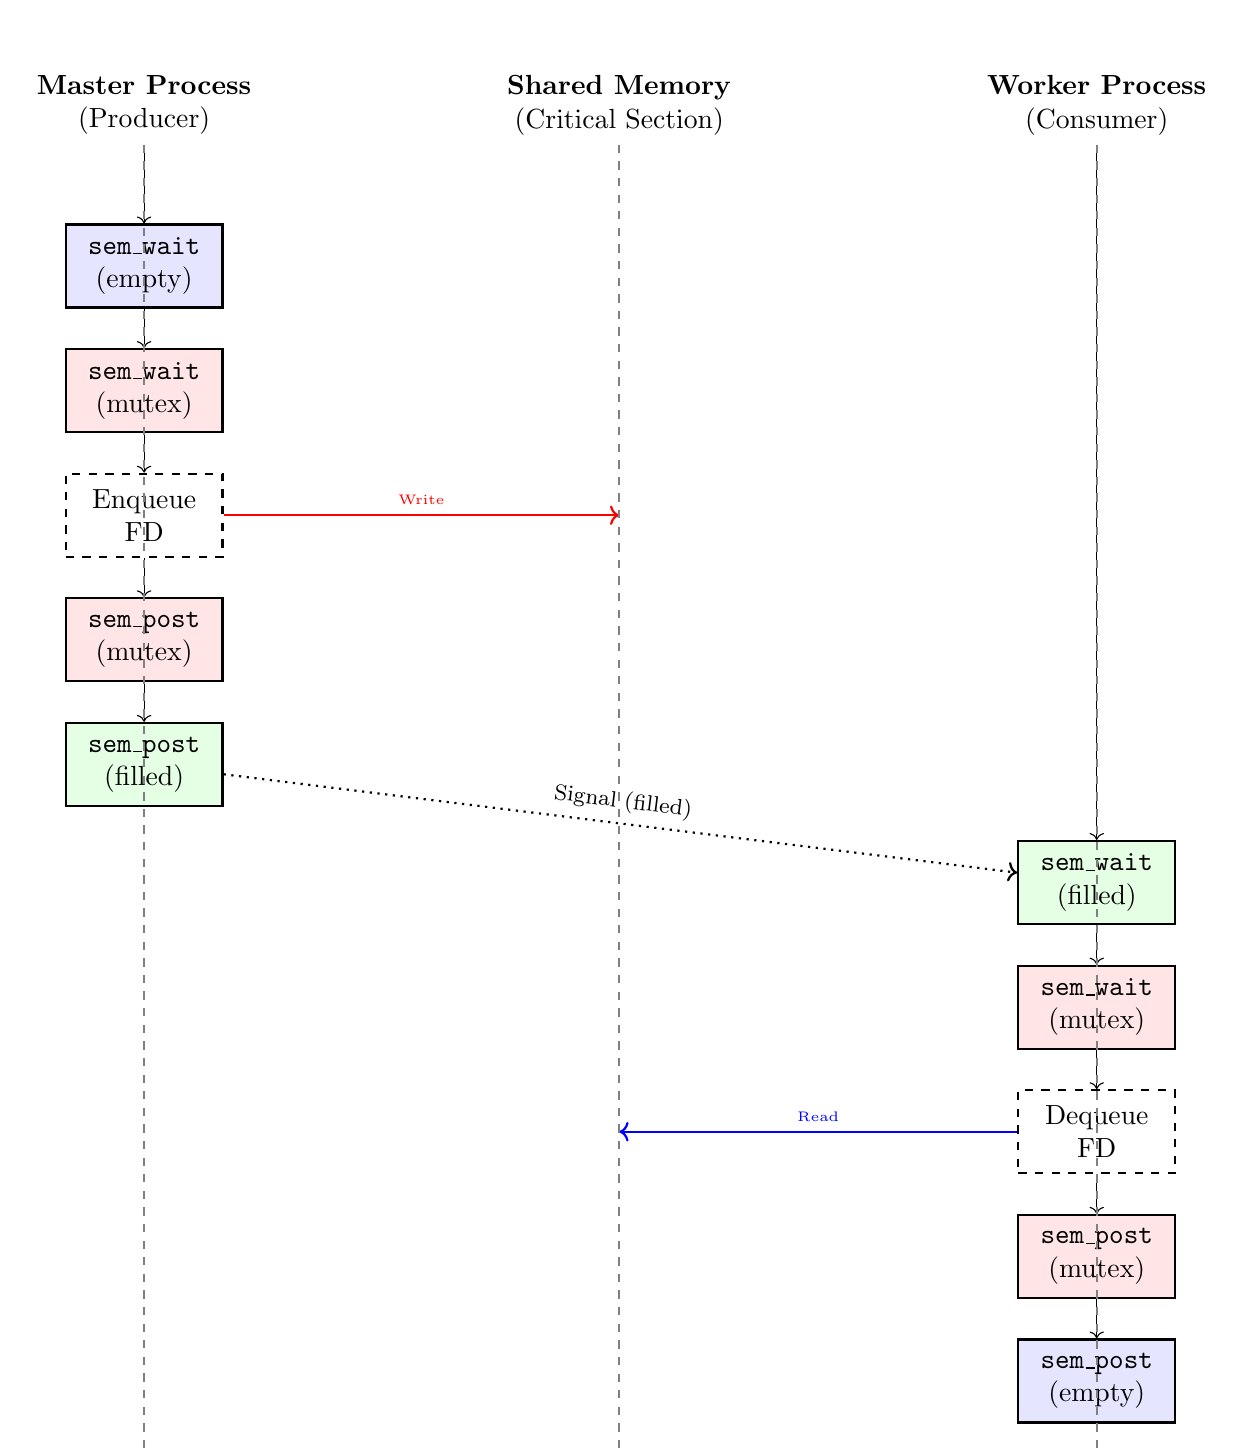
\begin{tikzpicture}[
            node distance=1.5cm,
            auto,
            block/.style={rectangle, draw=black, thick, fill=white, text width=5em, align=center, minimum height=3em},
            line/.style={draw, thick, -latex, shorten >=2pt},
            comment/.style={text width=4cm, align=left, gray, font=\footnotesize}
        ]
        
        % --- Columns ---
        \node (master) [align=center] {\textbf{Master Process} \\ (Producer)};
        \node (shm) [right=3cm of master, align=center] {\textbf{Shared Memory} \\ (Critical Section)};
        \node (worker) [right=3cm of shm, align=center] {\textbf{Worker Process} \\ (Consumer)};

        % --- Master Flow ---
        \node[block, fill=blue!10, below=1cm of master] (m_wait) {\texttt{sem\_wait}\\(empty)};
        \node[block, fill=red!10, below=0.5cm of m_wait] (m_lock) {\texttt{sem\_wait}\\(mutex)};
        \node[block, dashed, below=0.5cm of m_lock] (m_write) {Enqueue FD};
        \node[block, fill=red!10, below=0.5cm of m_write] (m_unlock) {\texttt{sem\_post}\\(mutex)};
        \node[block, fill=green!10, below=0.5cm of m_unlock] (m_signal) {\texttt{sem\_post}\\(filled)};

        % --- Worker Flow (offset down) ---
        \node[block, fill=green!10] (w_wait) at ($(worker |- m_signal) + (0,-1.5)$) {\texttt{sem\_wait}\\(filled)};
        \node[block, fill=red!10, below=0.5cm of w_wait] (w_lock) {\texttt{sem\_wait}\\(mutex)};
        \node[block, dashed, below=0.5cm of w_lock] (w_read) {Dequeue FD};
        \node[block, fill=red!10, below=0.5cm of w_read] (w_unlock) {\texttt{sem\_post}\\(mutex)};
        \node[block, fill=blue!10, below=0.5cm of w_unlock] (w_signal) {\texttt{sem\_post}\\(empty)};

        % --- Arrows interacting with Critical Section ---
        \draw[->, thick, red] (m_write.east) -- node[above, font=\tiny] {Write} (shm |- m_write);
        \draw[<-, thick, blue] (shm |- w_read) -- node[above, font=\tiny] {Read} (w_read.west);

        % --- Sequence Lines ---
        \draw[->] (master) -- (m_wait);
        \draw[->] (m_wait) -- (m_lock);
        \draw[->] (m_lock) -- (m_write);
        \draw[->] (m_write) -- (m_unlock);
        \draw[->] (m_unlock) -- (m_signal);

        \draw[->] (worker) -- (w_wait);
        \draw[->] (w_wait) -- (w_lock);
        \draw[->] (w_lock) -- (w_read);
        \draw[->] (w_read) -- (w_unlock);
        \draw[->] (w_unlock) -- (w_signal);

        % --- Cross-Process Signal ---
        \draw[->, dotted, thick] (m_signal) -- node[above, sloped, font=\footnotesize] {Signal (filled)} (w_wait);

        % --- Time lines (drawn last) ---
        \path (w_signal.south) ++(0,-0.5) coordinate (bottom_y);
        \draw[thick, gray, dashed] (master) -- (master |- bottom_y);
        \draw[thick, gray, dashed] (shm) -- (shm |- bottom_y);
        \draw[thick, gray, dashed] (worker) -- (worker |- bottom_y);

\end{tikzpicture}%
}
\caption{Producer-Consumer Synchronization Logic preventing Deadlocks}
\label{fig:sync_logic}
\end{figure}
    \subsection{Thread Synchronization (Mutex \& Condition Variables)}
    Inside each Worker, the thread pool uses in-process primitives (see \texttt{thread\_pool.h/.c}):
    
    \begin{itemize}
      \item \textbf{\texttt{pthread\_mutex\_t}} — protects the internal job queue and shared pool state.
      \item \textbf{\texttt{pthread\_cond\_t}} — allows worker threads to sleep when the queue is empty and wake on job submission or shutdown.
    \end{itemize}
    
    Threads block on \texttt{pthread\_cond\_wait} when there is no work. They are released by \texttt{pthread\_cond\_signal} or \texttt{pthread\_cond\_broadcast} on submission or shutdown, ensuring stable throughput without busy-waiting.
    
    % ----------------------------------------------------------------------
    % 4. COMPONENT DESIGN
    % ----------------------------------------------------------------------
    \section{Component Design}
    
    \subsection{LRU Cache}
    
    Each Worker maintains an in-memory Least Recently Used (LRU) cache for static file
    contents, combining a hash table (for $O(1)$ lookups) with a doubly linked list
    (for recency order). Capacity is enforced in bytes; entries in active use are
    protected from eviction via reference counting.
    
    \paragraph{Structures.}\mbox{}\\[-0.2\baselineskip]
    \begin{lstlisting}[language=C]
    // Cache entry: path key, raw data, size, list links, bucket link, refcount
    typedef struct cache_entry {
        char *key;                  
        uint8_t *data;               
        size_t size;                
        struct cache_entry *prev, *next;  
        struct cache_entry *hnext;       
        size_t refcnt;               
    } cache_entry_t;
    
    // Cache container: capacity/accounting, LRU ends, hash table, RW lock, stats
    struct file_cache {
        size_t capacity;              
        size_t bytes_used;            
        size_t items;                 
        cache_entry_t *lru_head;      
        cache_entry_t *lru_tail;     
        size_t nbuckets;             
        cache_entry_t **buckets;    
        pthread_rwlock_t rwlock;     
        size_t hits, misses, evictions; 
    };
    \end{lstlisting}
    
    \paragraph{Concurrency.}
    The cache is protected by \texttt{pthread\_rwlock\_t}: lookups acquire the read
    lock; insertions, updates, and evictions acquire the write lock. This enables
    high read concurrency while preserving exclusive access for structural changes.
    
    \paragraph{Operation.}\mbox{}\\[-0.2\baselineskip]
    \texttt{cache\_get(key)} computes the bucket, scans for a matching entry, and on
    hit promotes it to the LRU head. On miss, the Worker loads the file, then
    \texttt{cache\_put(key, data, size)} inserts the entry, updating
    \texttt{bytes\_used}. If capacity is exceeded, the cache evicts from the LRU tail
    until within limit; entries with \texttt{refcnt>0} are skipped. Oversized files
    may be served but not cached.
    
    \paragraph{Integration.}\mbox{}\\[-0.2\baselineskip]
    Workers consult the cache before disk I/O. On hit/miss, they update the cache
    counters and the shared system statistics accordingly. Because each Worker owns
    its cache, no inter-process locking is required; only per-cache RW locking
    applies.
    
    
    % ----------------------------------------------------------------------
    \subsection{Thread-Safe Logging}
    
    All processes append to a single log. Writes are serialized with a named POSIX semaphore and the file is opened with \texttt{O\_APPEND} to ensure atomic append.
    
    \paragraph{API.}\mbox{}\\[-0.2\baselineskip]
    The logger records structured entries via:
    \begin{lstlisting}[language=C]
    void logger_write(const char* ip,
                      const char* method,
                      const char* path,
                      int status,
                      size_t bytes_sent,
                      long duration_ms);
    \end{lstlisting}
    Each call emits a single line containing client IP, method, path, status, response size, and request latency.
    
    \paragraph{Synchronization.}\mbox{}\\[-0.2\baselineskip]
    A named semaphore (\texttt{sem\_open}, initial value 1) guards the critical section:
    \begin{itemize}
      \item \texttt{sem\_wait(g\_sem)} before formatting/buffering;
      \item optional buffered accumulation; periodic/time-based flush;
      \item rotation check; atomic \texttt{write}/\texttt{fflush};
      \item \texttt{sem\_post(g\_sem)} on exit.
    \end{itemize}
    Using \texttt{O\_APPEND} guarantees kernel-level append semantics even if multiple processes hold the file descriptor.
    
    \paragraph{Rotation \& Buffering.}\mbox{}\\[-0.2\baselineskip]
    The logger maintains an internal buffer and rotates the file at about 10\,MB, keeping a finite number of generations. A time-based flush (e.g., 5\,s) reduces syscall frequency without relaxing mutual exclusion.
    
    \paragraph{Integration.}\mbox{}\\[-0.2\baselineskip]
    The Master logs accepts and lifecycle events; Workers log per-request lines with latency. This yields stable, non-interleaved audit trails suitable for throughput/latency analysis and error triage.
    
    
    % ----------------------------------------------------------------------
    \subsection{Summary}
    
    \begin{table}[H]
    \centering
    \small
    \begin{tabular}{|l|l|p{5.5cm}|}
    \hline
    \textbf{Component} & \textbf{Synchronization} & \textbf{Purpose} \\ \hline
    Cache & \texttt{pthread\_rwlock\_t} & Multi-reader/single-writer protection for static file caching. \\ \hline
    Logger & \texttt{sem\_t *} & Serializes log file access across all processes. \\ \hline
    Threaded Logger & \texttt{mutex + cond\_t} & Async batched logging for reduced I/O contention. \\ \hline
    \end{tabular}
    \caption{Component Synchronization Summary}    

    \end{table}


    \subsection{Real-time Statistics Dashboard (Bonus)}

    The server implements a dedicated API endpoint at \texttt{/api/stats}. 
    Unlike static file serving, this endpoint bypasses the disk cache and reads directly from the global \texttt{server\_stats\_t} structure in shared memory.

    The architecture supports a JavaScript-based dashboard (\texttt{dashboard.html}) that polls this endpoint, rendering real-time graphs of throughput and latency. 
    
    % ----------------------------------------------------------------------
    % 5. SYSTEM LIFECYCLE
    % ----------------------------------------------------------------------
    \section{System Lifecycle}
    
    \subsection{Initialization}
    At startup, the Master process loads configuration parameters from
    \texttt{server.conf}, then creates the required POSIX shared memory region and
    named semaphores that enable communication and synchronization across processes.
    It proceeds to initialize the TCP listening socket and fork the configured number of
    Worker processes. Each Worker attaches to the existing shared memory and semaphores,
    initializes its local components (cache, logger, and thread pool), and waits for tasks
    to arrive through the interprocess queue.
    
    \subsection{Steady Operation}
    During normal execution, the Master continuously accepts new client connections and
    enqueues them into the shared circular buffer. Each Worker dequeues available requests,
    dispatching them to a thread pool that handles HTTP parsing, response generation, cache
    lookup, and logging. Shared statistics are updated atomically under semaphore
    protection. This design ensures high concurrency while maintaining strict consistency
    of shared state.
    
    \subsection{Graceful Shutdown}
    When receiving a termination signal (\texttt{SIGINT} or \texttt{SIGTERM}), the Master
    stops accepting new connections and signals all Workers to exit. Each Worker halts its
    dispatch loop, terminates its thread pool after completing active requests, and releases
    local resources. Finally, the Master process waits for all Workers to terminate and then
    cleans up global IPC objects, including shared memory segments and named semaphores,
    before exiting cleanly.
    
    \subsection{Error Recovery}
    If initialization or runtime failures occur—such as socket binding errors, semaphore
    creation issues, or shared memory faults—the system logs the event, cleans any partially
    allocated resources, and exits with an appropriate status code to prevent IPC leakage.
    
    
    % ----------------------------------------------------------------------
    % 6. DIAGRAMS
    % ----------------------------------------------------------------------
    \section{Flowcharts}
    % [Instruction: Add required flowcharts here]
    
\begin{figure}[H]
    \centering
    \resizebox{0.95\textwidth}{!}{%
    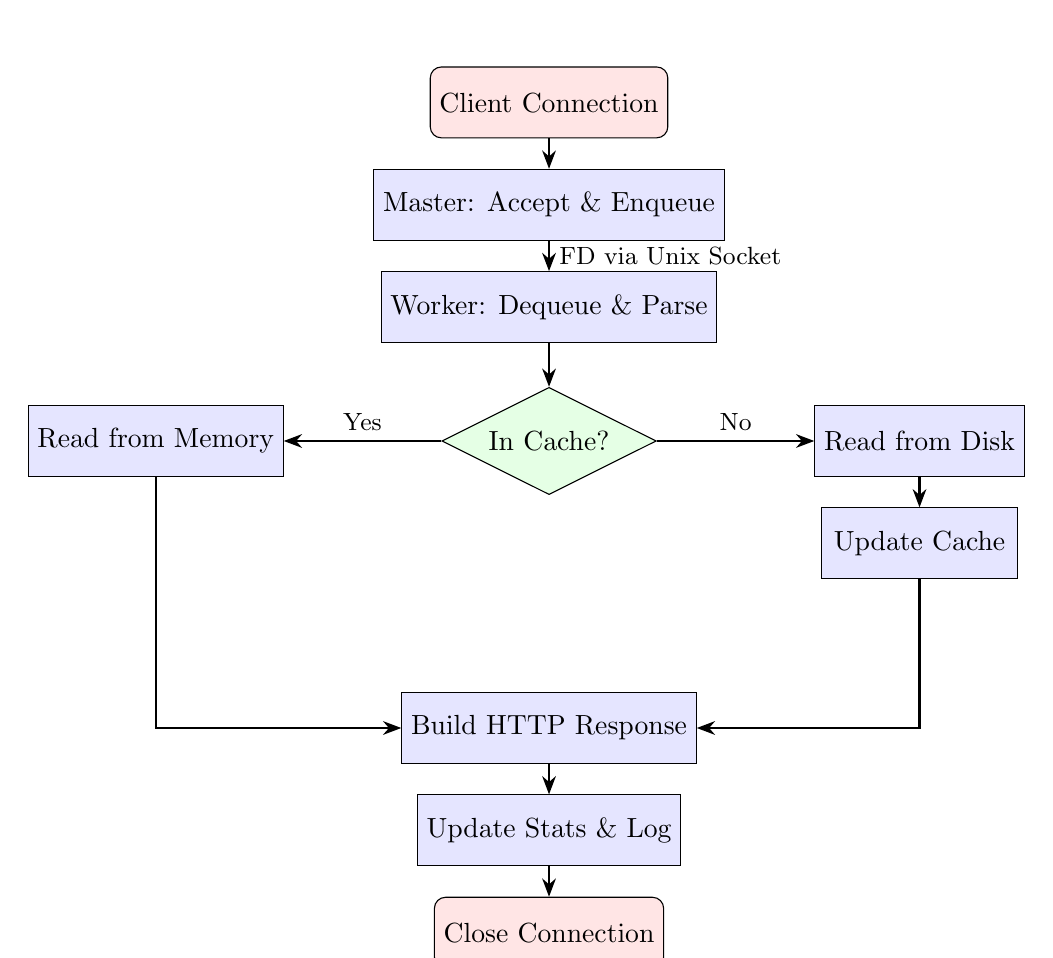
\begin{tikzpicture}[
        node distance=1.3cm,
        startstop/.style={rectangle, rounded corners, minimum width=2.5cm, minimum height=0.9cm, text centered, draw=black, fill=red!10},
        process/.style={rectangle, minimum width=2.5cm, minimum height=0.9cm, text centered, draw=black, fill=blue!10},
        decision/.style={diamond, minimum width=2.5cm, minimum height=0.9cm, text centered, draw=black, fill=green!10, aspect=2},
        arrow/.style={thick,->,>=Stealth}
    ]

    % --- NODES ---
    \node (start) [startstop] {Client Connection};
    \node (accept) [process, below of=start] {Master: Accept \& Enqueue};
    \node (worker) [process, below of=accept] {Worker: Dequeue \& Parse};
    \node (decide) [decision, below of=worker, yshift=-0.4cm] {In Cache?};
    
    % 5. Branches
    \node (read_disk) [process, right=2cm of decide] {Read from Disk};
    \node (update_cache) [process, below of=read_disk] {Update Cache};
    \node (read_mem) [process, left=2cm of decide] {Read from Memory};
    
    % 6. Response
    \node (build) [process, below=2.5cm of decide] {Build HTTP Response};
    \node (log) [process, below of=build] {Update Stats \& Log};
    \node (end) [startstop, below of=log] {Close Connection};

    % --- ARROWS ---
    \draw [arrow] (start) -- (accept);
    \draw [arrow] (accept) -- node[right, font=\small] {FD via Unix Socket} (worker);
    \draw [arrow] (worker) -- (decide);
    
    % Cache Miss Path
    \draw [arrow] (decide) -- node[above, font=\small] {No} (read_disk);
    \draw [arrow] (read_disk) -- (update_cache);
    \draw [arrow] (update_cache) |- (build);
    
    % Cache Hit Path
    \draw [arrow] (decide) -- node[above, font=\small] {Yes} (read_mem);
    \draw [arrow] (read_mem) |- (build);
    
    % Final Path
    \draw [arrow] (build) -- (log);
    \draw [arrow] (log) -- (end);

    \end{tikzpicture}%
    }
    \caption{Flowchart of an HTTP Request Lifecycle within the Server}
    \label{fig:flowchart}
\end{figure}
    
    \end{document}
